\documentclass[12pt,a4paper]{scrartcl}
\usepackage[utf8]{inputenc}
\usepackage[english,russian]{babel}
\usepackage{indentfirst}
\usepackage{misccorr}
\usepackage{graphicx}
\usepackage{amsmath}
\usepackage{multirow}
\usepackage{pgfplots}
\usepackage[top=1cm, bottom=1cm, left=1cm, right=1cm]{geometry}
\pgfplotsset{compat=1.9}

\begin{document}
	\graphicspath{{C:/Users/Alex/OneDrive/Изображения/TexImgs}}
	
	\newcommand{\ms}{\mathstrut}
	\newcommand{\msp}{\hspace{0.5cm}}
	\newcommand{\al}{\alpha}
	\newcommand{\dg}{^\circ}
	\newcommand{\qd}[2]{^{\frac{#1}{#2}}}
	\newcommand{\qdm}[2]{^{-\frac{#1}{#2}}}
	\newcommand{\lm}[2]{\underset{#1 \rightarrow #2}{\lim}}
	\newcommand{\sfrac}[2]{\dfrac{\strut #1}{\strut #2}}
	\newcommand{\equal}[1]{\overset{(#1)}{=}}
	\newcommand{\linevdots}{\ \raisebox{-.08\height}{\vdots}\ }
	\newcommand{\linecvdots}{\ \raisebox{-.08\height}{\vdots}\hspace{-0.13cm}\raisebox{.15\height}{\cancel{\phantom{a}}\hspace{0.06cm}}}
	\newcommand{\combox}[1]{\ms \msp \msp \begin{minipage}{0.95\linewidth}
			#1
	\end{minipage}}
	
	\newtheorem{pr}{Задача}
	\newtheorem{ex}{Пример}
	\newtheorem{dfn}{Def}
	\newtheorem{theorem}{Th}
	
	\newenvironment{slv}{\ms \msp \textit{Решение:}}{}
	\newenvironment{proof}{\ms \msp \textit{Доказательство: }}{\hfill $\square$}
	
	\begin{titlepage}
		
		\vspace*{\fill}
		
		\begin{center}
			
\includegraphics[scale=0.8]{MIPT.png}
			\\[0.7cm]\Huge Московский Физико-Технический Институт\\(национальный исследовательский университет)
			\\[2cm]\LARGE Отчет по эксперименту
			\\[0.5cm]\noindent\rule{\textwidth}{1pt}
			\\\Huge\textbf{Изучение экспериментальных погрешностей\\на примере физического маятника}
			\\[-0.5cm]\noindent\rule{\textwidth}{1pt}
		\end{center}
		
		\begin{flushleft}
			\textit{Работа №1.4.1; дата: 05.10.21}\hfill\textit{Семестр: 1}
		\end{flushleft}
		
		\vspace*{\fill}
		
		\begin{flushleft}
			Выполнил: \hspace{\fill} Группа:
			\\Кошелев Александр \hspace{\fill} Б05-105
		\end{flushleft}
	\end{titlepage}
	
	%Страница 2
	
	\begin{flushleft}
		\footnotesize{Изучение экспериментальных погрешностей на примере физического маятника} \hspace{\fill} \footnotesize{2}
		\\[-0.3cm]\noindent\rule{\textwidth}{0.3pt}
	\end{flushleft}

	\section{Аннотация}
	
	Данная работа посвящена изучению погрешностей, возникающих при экспериментальных измерениях.
	
	\textbf{Цель работы:}
	\begin{enumerate}
		\item  На примере измерения периода свободных колебаний физического
		маятника познакомиться с систематическими и случайными погрешностями, прямыми и косвенными измерениями;
		\item Проверить справедливость формулы для периода колебаний физического маятника и определить значение ускорения свободного падения;
		\item Убедиться в справедливости теоремы Гюйгенса об обратимости
		точек опоры и центра качания маятника;
		\item Оценить погрешность прямых и косвенных измерений и конечного результата.
	\end{enumerate}

	\textbf{В работе используются:} металлический стержень с опорной призмой; дополнительный груз; закреплённая на стене консоль; подставка с острой гранью для определения цента масс маятника; секундомер; счётчик колебаний (механический или
	электронный); линейки металлические различной длины; штангенциркуль; электронные весы; математический маятник (небольшой груз, подвешенный на нитях). 

	\section{Теоретические сведения}
	В курсе механики показывается, что момент инерции $J_{\text{с}}$ тонкого стержня массой $m$ и длины $l$, вращающегося вокруг оси, проходящей через центр масс:
	\begin{equation}
		J = \sfrac{ml^2}{12}
	\end{equation}

	При помощи теоремы Гюйгенса-Штейнера из уравнения (1) можно получить момент инерции $J$ для стержня, подвешенного на расстоянии $a$ от центра:
	\begin{equation}
		J = \sfrac{ml^2}{12} + ma^2
	\end{equation}

	Получим формулу для периода колебаний физического маятника из формулы для пружинного маятника $T = 2\pi\sqrt{m/k}$. Роль массы здесь играет момент инерции $J$, а роль коэффициента жесткости $k$ --- коэффициент между моментом силы и величиной отклонения. Таким образом:
	\begin{equation}
		T = 2\pi\sqrt{\sfrac{J}{mga}}
	\end{equation}
	
	В нашем случае для стержня длины $l$, подвешенного на расстоянии $a$ от центра:
	\begin{equation}
		T = 2\pi\sqrt{\sfrac{\sfrac{l^2}{12} + a^2}{ga}}
	\end{equation}

	\newpage
	%Страница 3
	
	\begin{flushleft}
		\footnotesize{Изучение экспериментальных погрешностей на примере физического маятника} \hspace{\fill} \footnotesize{3}
		\\[-0.3cm]\noindent\rule{\textwidth}{0.3pt}
	\end{flushleft}

	Сформулируем понятие \textit{приведенной длины} физического маятника.
	\begin{dfn}
		Приведенной длиной физического маятника называется величина $$l_{\text{пр}} = a + \sfrac{l^2}{12a}$$
	\end{dfn}
	
	Смысл этой длины в том, что физический маятник длины $l$, подвешенный
	в точке $a$, имеет тот же период малых колебаний, что и математический
	маятник длиной $l_{\text{пр}}$. Сформулируем важную теорему.
	\begin{figure}[h]
		\begin{minipage}{0.7\linewidth}
			\begin{theorem}[Гюйгенса]
				Рассмотрим точку $OO'$, отстоящую от точки опоры $OO$ на расстояние $l_{\text{пр}}$ вдоль стержня (эту точку иногда называют центром качания физического маятника). Оказывается, если маятник подвесить за точку $O'$, то период его качания не изменится. Иными словами, точка опоры и центр качания маятника взаимно обратимы.
			\end{theorem}			
		\end{minipage}
		\begin{minipage}{0.3\linewidth}
			\begin{center}
				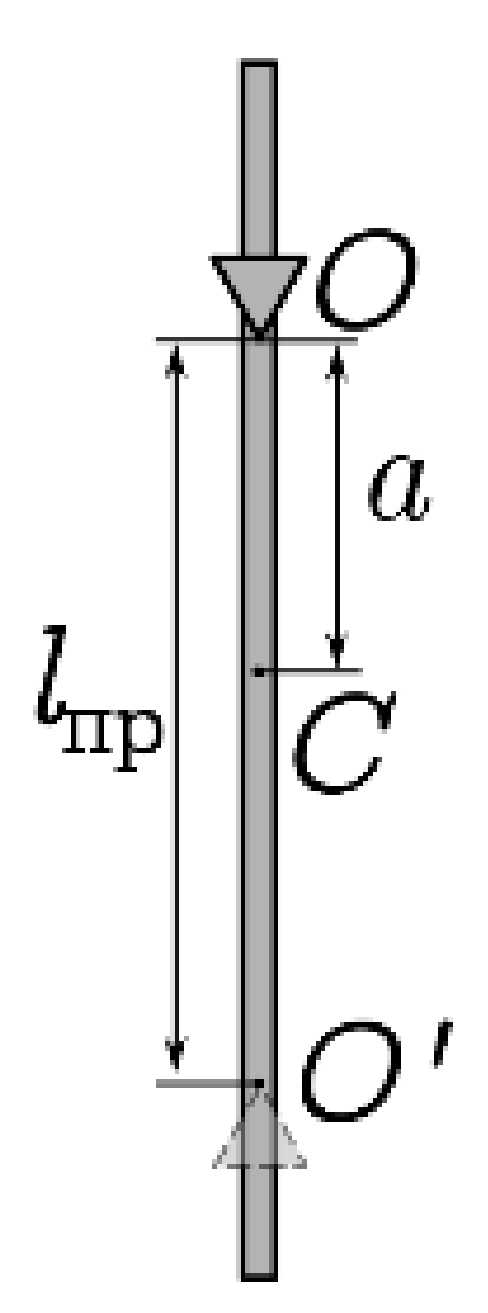
\includegraphics[scale=0.1]{PIC_1.png}
				\\\textbf{Рис. 1:} К теореме Гюйгенса
			\end{center}
		\end{minipage}
	\end{figure}



	Из динамики гармонических колебаний можно получить уравнение гармонических колебаний:

	$$\varphi(t) = A\sin(\Omega t + \alpha)$$

	где $\Omega = \sfrac{2\pi}{T} = \sqrt{\sfrac{mga}{l}}$ --- угловая частота колебаний, $A$ - угловая амплитуда, $\alpha$ - начальная фаза колебаний. Но данное уравнение справедливо только в идеальном случае, когда нет потерь энергии в коебательной системе. В реальности они всегда присутствуют, можно показать, что амплитуда от времени зависит экспоненциально ($\gamma$ - декремент затухания):

	$$A(t) = A_0e^{-\gamma t}$$

	

	В связи с этим принято использовать характеристику колебательной системы, называемую \textit{добротностью}:

	$$Q = \pi \sfrac{\tau_{\text{зат}}}{T}$$

	

	\section{Экспериментальная установка}

	Тонкий стальной стержень длиной $l \approx 1\,$м и массой $m \approx 1\,$кг (точные параметры определяются непосредственными измерениями) подвешивается на прикреплённой стене консоли с помощью небольшой призмы. Диаметр стержня много меньше его длины $d\approx 12\, \text{мм} \ll l$. Небольшая призма крепится на стержне винтом и острым основанием опирается на поверхность закреплённой на стене консоли. Острие ребра призмы образует ось качания маятника.

	Возможны две схемы реализации установок.

	

	\newpage

	%Страница 4

	

	\begin{flushleft}

		\footnotesize{Изучение экспериментальных погрешностей на примере физического маятника} \hspace{\fill} \footnotesize{4}
		\\[-0.3cm]\noindent\rule{\textwidth}{0.3pt}

	\end{flushleft}



	\paragraph{Установка А.} Призму можно перемещать вдоль стержня, изменяя длину $A$ --- расстояние от центра масс до точки подвеса. Период колебаний измеряется непосредственно с помощью секундомера.

	

	\paragraph{Установка B.} Подвесная призма остаётся неподвижной ($a = const$), а на стержень маятника насаживается дополнительное тело небольшого размера («чечевица» или цилиндр), положение которого можно изменять, изменяя таким образом момент инерции маятника. Период колебаний маятника в этой схеме измеряется электронным счетчиком импульсов, расположенным у нижнего конца стержня.

	

	Расстояния во всех установках измеряются линейками и штангенциркулем. Положение центра масс маятника может быть определено с помощью балансирования маятника на вспомогательной $\perp$-образной подставке с острой верхней гранью.

	

	Измеряя зависимости периода малых колебаний от положения стержня или дополнительного тела на нём, можно экспериментально проверить формулу (3) (или её частный случай (4)) и вычислить значение ускорения свободного падения $g$. Формулу (4) можно проверить, откладывая по осям величины $u = T^2 a$ и $v = a^2$ . В этих координатах график $u(v)$ должен иметь вид прямой линии, угловой коэффициент которой пропорционален $g$, а вертикальное смещение --- моменту инерции стержня относительно центра масс.
	
	\section{Измерение времени секундомером}
	
	Измерение периода колебаний маятника (и любых других промежутков времени) с помощью секундомера неизбежно сопровождается погрешностью из-за конечного времени реакции человека. Как правило, время реакции составляет $0.1-0.2\,$с. Однако это время различно для разных людей и зависит от большого числа субъективных факторов (состояние человека, тренированность, время суток, освещённость и т.п.). Для планирования эксперимента и для корректной оценки его погрешностей следует иметь
	более точное значение погрешности измерения времени.
	
	Найти случайную погрешность из-за времени реакции (а также из-за других сопутствующих случайных факторов) нетрудно экспериментально. Для этого достаточно несколько раз повторить опыт по измерению одного и того же числа колебаний маятника. По полученному набору результатов $\{t_1, t_2, ..., t_N\}$ определить среднее значение $\overline{t}$ и среднеквадратичное отклонение отдельного измерения:
	\begin{equation}
		\sigma_t^{\text{случ}} = \sqrt{\sfrac{1}{N - 1}\sum(t_i - \overline{t})^2}
	\end{equation}
	Кроме того, у каждого секундомера возможна систематическая погрешность $\sigma_t^{\text{сист}}$, максимальная величина которой устанавливается производителем (определить её можно по маркировке на приборе или по его паспорту). Как правило у секундомера есть погрешность цены деления (или погрешность округления у цифрового секундомера), а также систематическая погрешность из-за постепенного «ухода» показаний с течением времени. Последняя зависит от класса точности секундомера: например, от лабораторных механических секундомеров 2-го класса точности следует ожидать погрешности $\sim 0.1\,$с за $60\,$с $(\sim 0.2\%)$. Полная погрешность измерения времени вычисляется среднеквадратично:
	\begin{equation}
		\sigma_t^{\text{полн}} = \sqrt{\left(\sigma_t^{\text{случ}}\right)^2 + \left(\sigma_t^{\text{сист}}\right)^2}
	\end{equation}
	При известной погрешности измерения времени $\sigma_t^{\text{полн}}$ можно спланировать проведение эксперимента исходя из требуемой точности опыта. В частности, можно определить, по какому количеству колебаний маятника следует измерять его период.
	
	\newpage
	
	%Страница 5
	
	
	
	\begin{flushleft}
		
		\footnotesize{Изучение экспериментальных погрешностей на примере физического маятника} \hspace{\fill} \footnotesize{5}
		\\[-0.3cm]\noindent\rule{\textwidth}{0.3pt}
		
	\end{flushleft}
	
	\section{Проведение эксперимента}
	\paragraph{Измерение длины стержня линейкой} \hfill
	
	\par Стержень располагается на столе, и к нему прикладывается линейка, начало линейки точно сопоставляется с началом стержня.
	$$l = (1001.0 \pm 0.5)\,\text{мм}\ \text{при}\ \varepsilon_l = 0.05\%$$
	
	\paragraph{Измерение центра масс} \hfill
	
	\par Определим координату центра масс, полагая ноль на конце с отверстием.
	$$l_c = (500.0 \pm 0.5)\,\text{мм}\ \text{при}\ \varepsilon_{l_c} = 0.1\%$$
	
	\paragraph{Измерение массы стержня} \hfill
	
	\par Масса стержня измеряется при помощи электронных весов.
	$$m_{\text{ст}} = (868.5 \pm 0.1)\,\text{г}\ \text{при}\ \varepsilon_{m_{\text{ст}}} = 0.01\%$$
	
	\paragraph{Измерение массы опорной призмы} \hfill
	
	\par Масса опорной призмы измеряется при помощи электронных весов.
	$$m_{\text{пр}} = (73.7 \pm 0.1)\,\text{г}\ \text{при}\ \varepsilon_{l_{пр}} = 0.1\%$$
	
	\paragraph{Оценка погрешности измерения времени} \hfill
	
	\par Произведем пробную серию замеров суммарного периода $N = 10$ колебаний.
	\begin{center}
		\begin{tabular}{|c|c|c|c|c|c|c|c|c|c|c|}
			\hline $i$ & 1 & 2 & 3 & 4 & 5 & 6 & 7 & 8 & 9 & 10
			\\\hline $t_i,\,$с & 15.99 & 15.37 & 15.48 & 15.48 & 15.51 & 15.50 & 15.47 & 15.99 & 15.71 & 15.61
			\\\hline $\overline{t},\,$с & \multicolumn{10}{|c|}{15.61}
			\\\hline $\sigma_t,\,$с & \multicolumn{10}{|c|}{0.22}
			\\\hline $\varepsilon_t$ & \multicolumn{10}{|c|}{0.014}
			\\\hline
		\end{tabular}
		\\\textbf{Табл. 1: Пробный замер}
	\end{center}
	\par Зададим планку погрешности измерения периода $\varepsilon_T = 0.0025\ (0.25\%)$, тогда:
	$$n = \sfrac{\sigma_t}{T\varepsilon_T} \approx 50$$
	
	\paragraph{Пробное измерение ускорения свободного падения} \hfill
	
	\par Замер при оценке погрешности времени производился при $a = 390\,$мм. Тогда грубая оценка получаемой величины:
	$$g \approx 9.8\,\sfrac{\text{м}}{\text{с}^2}$$
	
	Таким образом, точность удовлетворительна, ведь полученное значение близко к табличному. А значит можно переходить к дальнейшим измерениям.
	
	\newpage
	
	%Страница 6
	
	
	
	\begin{flushleft}
		
		\footnotesize{Изучение экспериментальных погрешностей на примере физического маятника} \hspace{\fill} \footnotesize{6}
		\\[-0.3cm]\noindent\rule{\textwidth}{0.3pt}
		
	\end{flushleft}
	
	\paragraph{Оценка ускорения свободного падения методом усреднения} \hfill
	
	\par Проведем серию экспериментов для определения ускорения свободного падения, рассчитаем также погрешности при этом.
	
	\begin{center}
		\begin{tabular}{|c|c|c|c|c|c|}
			\hline № & $a,\,$cм & $n$ & $t_i,\,$с & $T_i,\,$с & $g,\,$м/с$^2$
			\\\hline 1 & 3.0 $\pm$ 0.5 & 50 & 169.18 $\pm$ 0.20 & 3.384 $\pm$ 0.004 & 9.86 $\pm$ 0.02
			\\\hline 2 & 5.0 $\pm$ 0.5 & 50 & 131.64 $\pm$ 0.20 & 2.633 $\pm$ 0.004 & 9.79 $\pm$ 0.01
			\\\hline 3 & 10.0 $\pm$ 0.5 & 50 & 97.25 $\pm$ 0.20 & 1.945 $\pm$ 0.004 & 9.76 $\pm$ 0.01
			\\\hline 4 & 15.0 $\pm$ 0.5 & 50 & 84.16 $\pm$ 0.20 & 1.683 $\pm$ 0.004 & 9.85 $\pm$ 0.01
			\\\hline 5 & 20.0 $\pm$ 0.5 & 50 & 79.06 $\pm$ 0.20 & 1.581 $\pm$ 0.004 & 9.75 $\pm$ 0.01
			\\\hline 6 & 25.0 $\pm$ 0.5 & 50 & 76.64 $\pm$ 0.20 & 1.533 $\pm$ 0.004 & 9.81 $\pm$ 0.01
			\\\hline 7 & 27.0 $\pm$ 0.5 & 50 & 76.59 $\pm$ 0.20 & 1.532 $\pm$ 0.004 & 9.74 $\pm$ 0.01
			\\\hline 8 & 29.0 $\pm$ 0.5 & 50 & 76.57 $\pm$ 0.20 & 1.531 $\pm$ 0.004 & 9.74 $\pm$ 0.01
			\\\hline 9 & 30.0 $\pm$ 0.5 & 50 & 76.31 $\pm$ 0.20 & 1.526 $\pm$ 0.004 & 9.81 $\pm$ 0.01
			\\\hline 10 & 32.0 $\pm$ 0.5 & 50 & 76.61 $\pm$ 0.20 & 1.532 $\pm$ 0.004 & 9.77 $\pm$ 0.01
			\\\hline 11 & 35.0 $\pm$ 0.5 & 50 & 76.76 $\pm$ 0.20 & 1.535 $\pm$ 0.004 & 9.86 $\pm$ 0.01
			\\\hline 12 & 40.0 $\pm$ 0.5 & 50 & 78.44 $\pm$ 0.20 & 1.569 $\pm$ 0.004 & 9.76 $\pm$ 0.01
			\\\hline 13 & 45.0 $\pm$ 0.5 & 50 & 79.95 $\pm$ 0.20 & 1.599 $\pm$ 0.004 & 9.81 $\pm$ 0.01
			\\\hline
		\end{tabular}
		\\\textbf{Табл. 2: Измерение ускорения свободного падения}
	\end{center}

	Усредним полученные значения ускорения свободного падения, итак:
	$$g = (9.80 \pm 0.01)\ \text{м}/\text{с}^2$$
	
	\paragraph{Определение точки минимума периода колебаний} \hfill
	\par Теоретически оценим точку минимума периода колебаний. Это несложно установить из формулы приведенной длины и формулы периода колебаний математического маятника.
	$$a_{min} \approx 29\,\text{см}$$
	
	\par Построим график зависимости $T(a)$, проверим наличие минимума и сравним его с теоретическим значением.
	
	\begin{center}
		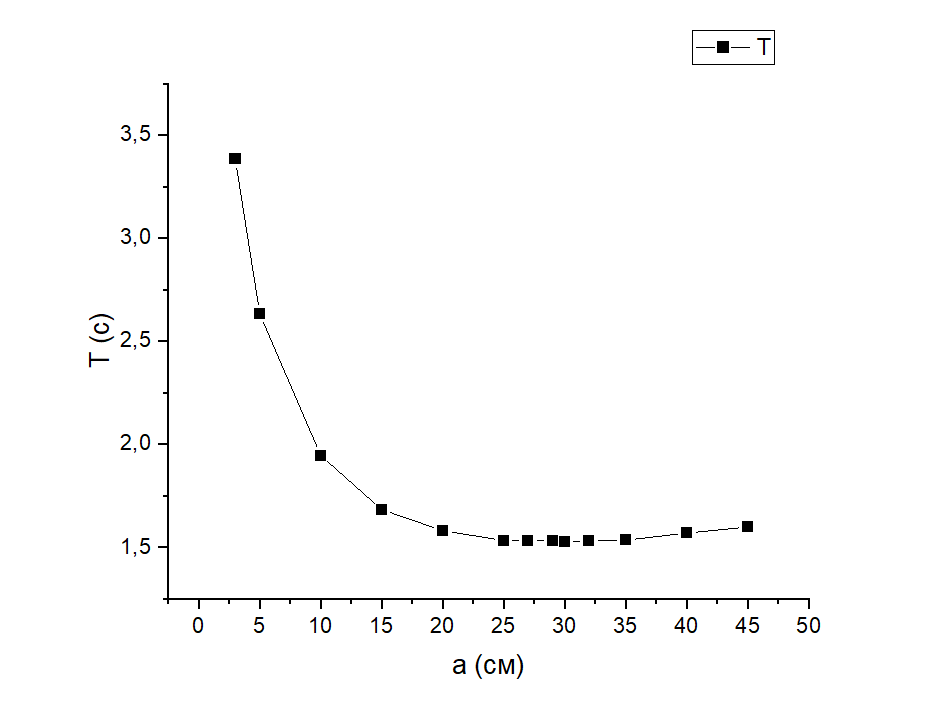
\includegraphics[scale=1.1]{PIC_2.png}
		\\\textbf{Рис. 2: График $T(a)$}
	\end{center}

	\par В самом деле график имеет минимум. Можно прикинуть, что он достигается именно около $a = 29\,$см.
	
	\newpage
	
	%Страница 7
	
	
	
	\begin{flushleft}
		
		\footnotesize{Изучение экспериментальных погрешностей на примере физического маятника} \hspace{\fill} \footnotesize{7}
		\\[-0.3cm]\noindent\rule{\textwidth}{0.3pt}
		
	\end{flushleft}
	
	\paragraph{Определение ускорения свободного падения методом наименьших квадратов} \hfill
	
	\par Построим график зависимости $a^2(T^2a)$. В соответствии с формулой для периода колебаний физического маятника, график должен получиться линейным с коэффициентом наклона $k = \frac{g}{4\pi^2}$.
	
	\begin{center}
		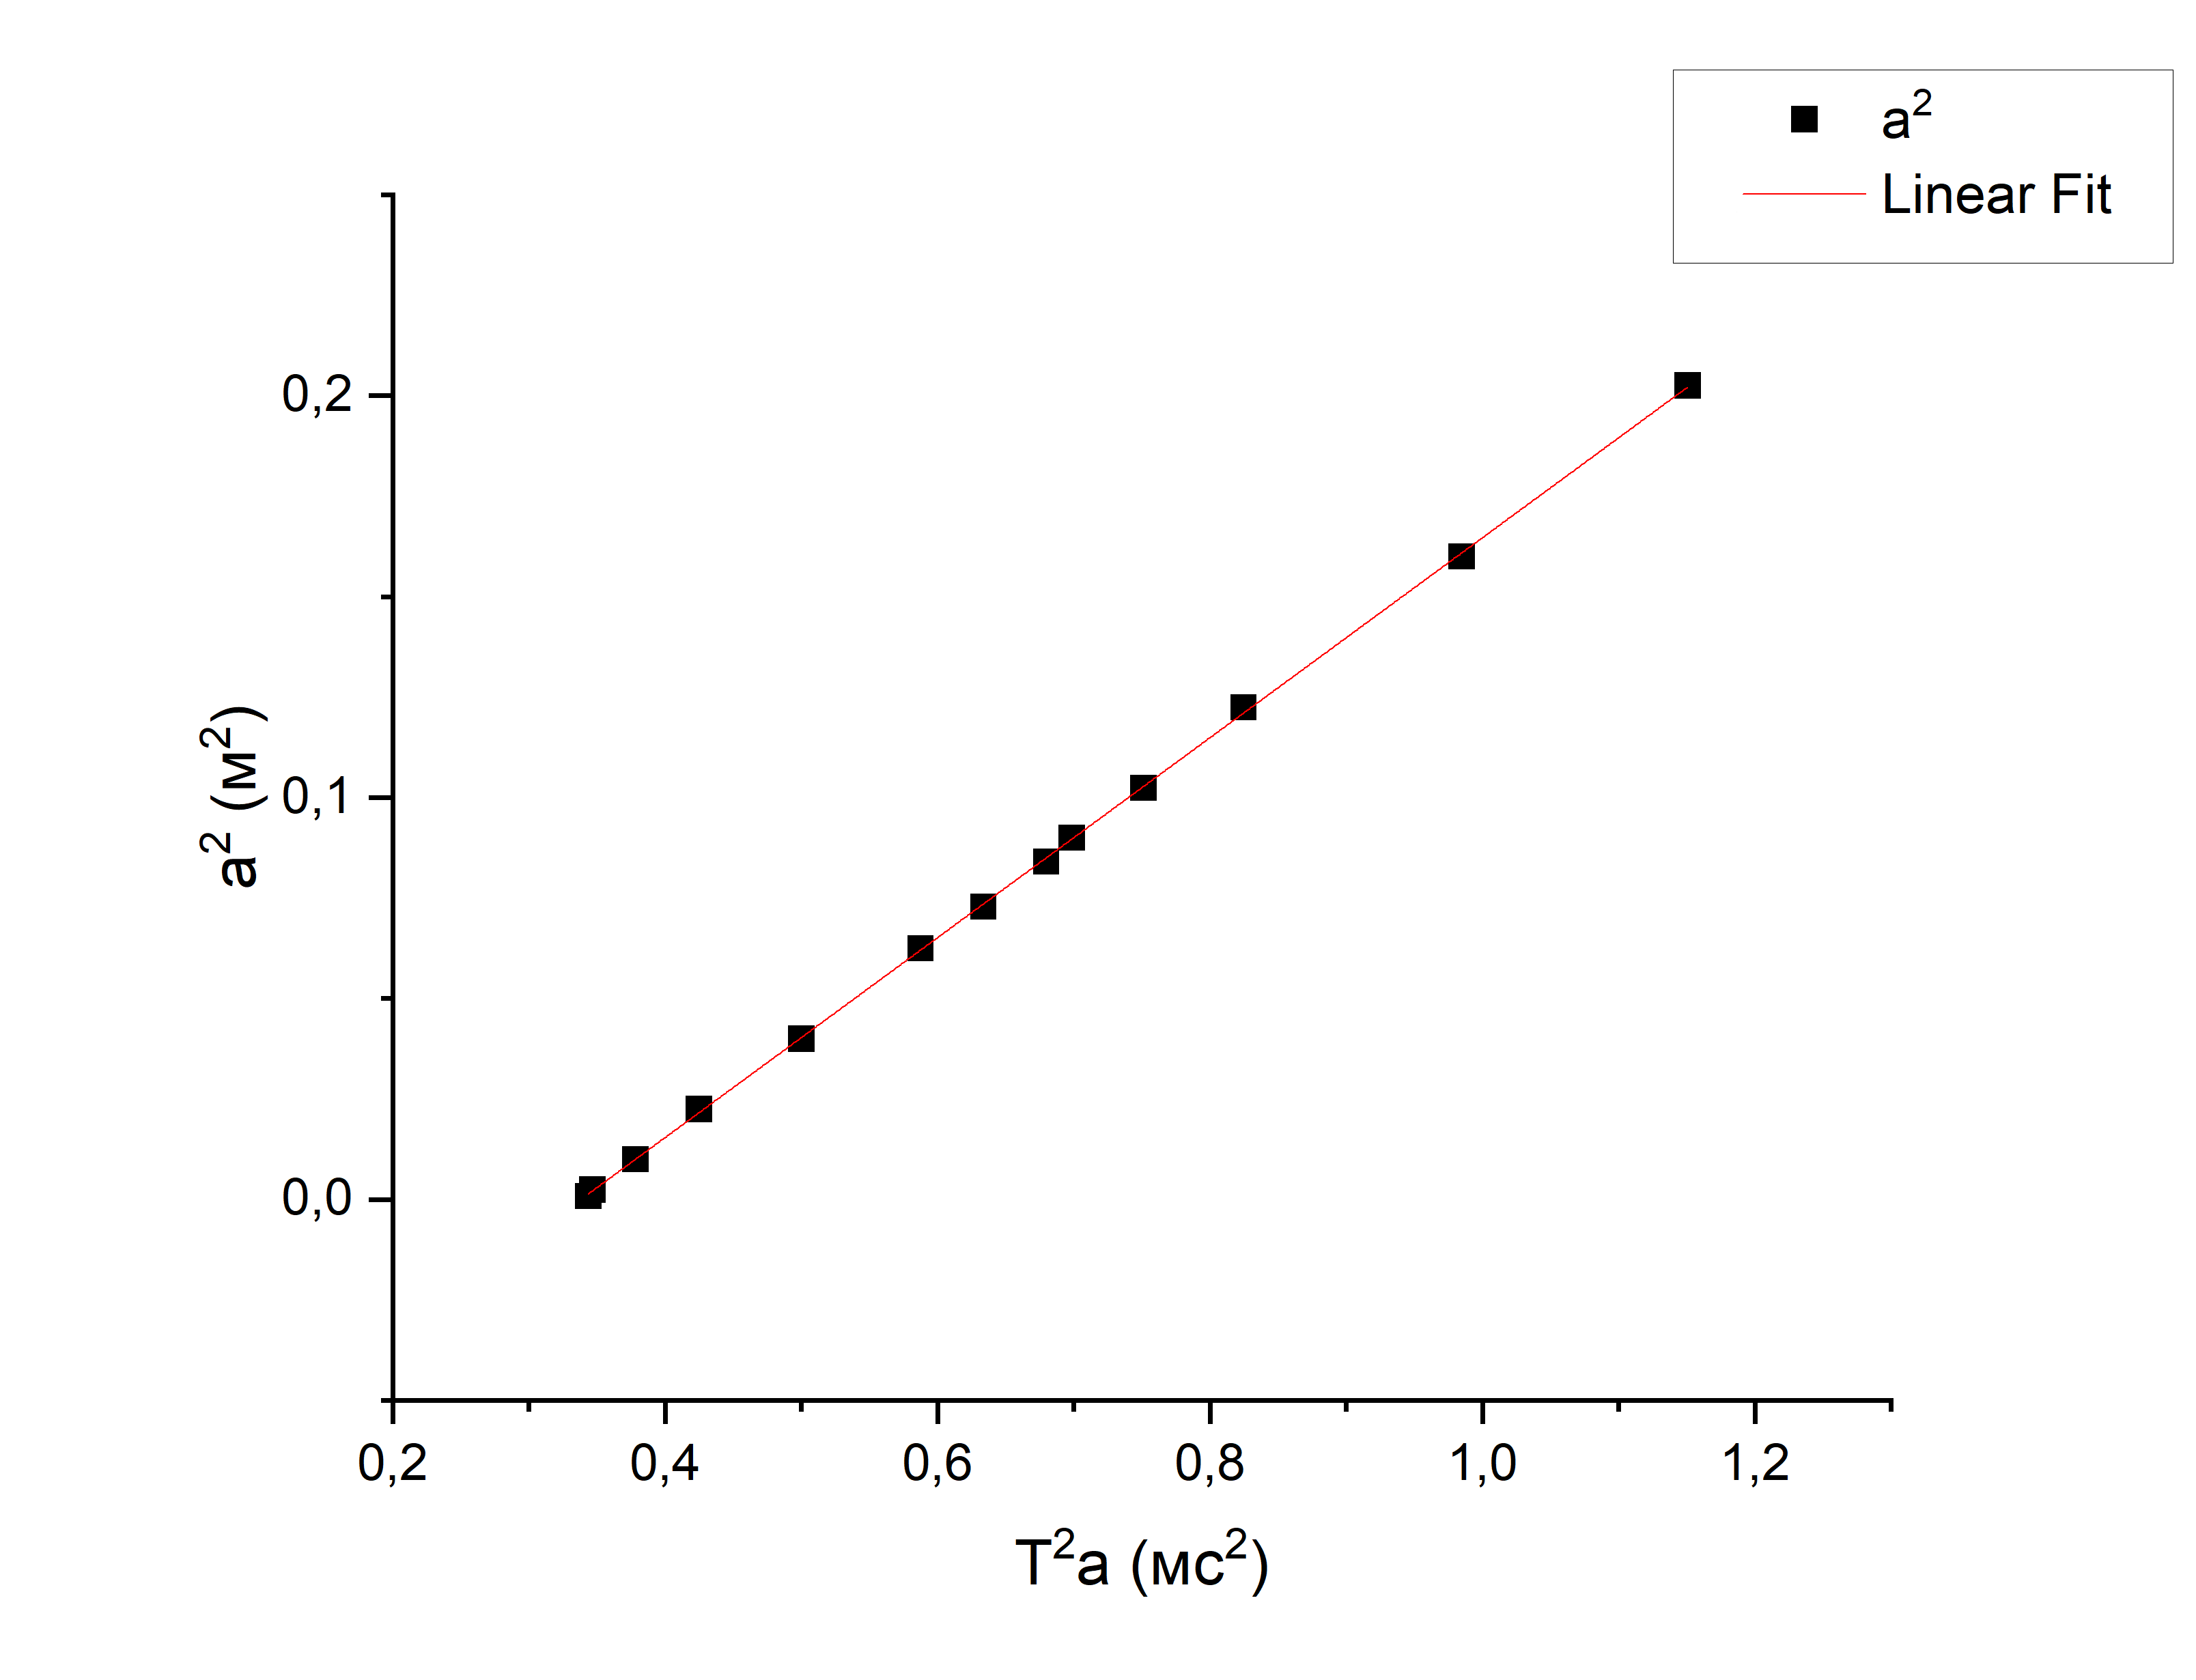
\includegraphics[scale=0.3]{PIC_3.png}
		\\\textbf{Рис. 3: График $a^2(T^2a)$}
	\end{center}

	Точки действительно ложатся с хорошей точностью на прямую. При помощи метода наименьших квадратов построим аппроксимирующую прямую. Представим ее в виде $y = kx + b$, тогда:
	$$k = (0.2487 \pm 0.0008)\,\text{м}/\text{с}^2$$
	$$b = (0.0840 \pm 0.0006)\,\text{м}^2$$
	
	И, наконец, по данному коэффициенту наклона:
	$$g = (9.82 \pm 0.03)\,\text{м}/\text{с}^2\ \text{при}\ \varepsilon_g = 0.3\%$$
	
	\paragraph{Проверка формулы для длины математического маятника} \hfill
	
	Рассчитаем приведенную длину для значения $a = 0.20\,$м. Тогда приведенная длина:
	$$l_{\text{пр}} \approx 0.62\,\text{м}$$
	
	Соответствующий период колебаний математического маятника данной длины по соответствующей формуле:
	$$T = 2\pi\sqrt{\sfrac{l}{g}} \approx 1.580\,\text{с}$$
	
	Данный период совпадает с физическим маятником, значение периода которого по эксперименту $(1.581 \pm 0.004)\,\text{с}$. На поверку, для других значений $a$ данное равенство тоже выполняется, из чего можно сделать вывод об истинности данной формулы.
	
	\paragraph{Проверка теоремы Гюйгенса} \hfill
	
	Поскольку центр масс стержня практически на середине, будем пользоваться таблицей нашего эксперимента для проверки. Рассмотрим для примера значение $a = 0.25\,$м. Соответствующее расстояние от центра масс $a' = l_{\text{пр}} - a \approx 0.32\,$м.
	Рассмотрим соответствующие периоды $T_a = (1.533 \pm 0.004)\,$с, $T_{a'} = (1.532 \pm 0.004)\,$с. С учетом погрешности эти значения совпадают с хорошей точностью. То же выполняется и для остальных значений $a$. Таким образом, теорему можно считать экспериментально доказанной.
	
	\newpage
	
	%Страница 8
	
	
	
	\begin{flushleft}
		
		\footnotesize{Изучение экспериментальных погрешностей на примере физического маятника} \hspace{\fill} \footnotesize{8}
		\\[-0.3cm]\noindent\rule{\textwidth}{0.3pt}
		
	\end{flushleft}
	
	\section{Выводы}
	В работе оценена точность измерения времени при помощи секундомера. Большую часть этой погрешности составляет человеческая реакция, определенное значение $\sigma_t = 0.2\,\text{с}$. Другие же измерения проводились весьма точно с небольшими относительными погрешностями, то есть измерения длин и масс частей маятника.

	В ходе эксперимента получено значение
	$$g = (9.82 \pm 0.03)\,\text{м}/\text{с}^2$$
	для ускорения свободного падения. Результат считаю хорошим, учитывая его близость к табличному значению, которое составляет $g_{\text{табл}} = (9.78 - 9.82)\,\text{м}/\text{с}^2$. Отдельно стоит отметить, что действительный результат лежит в рамках погрешности эксперимента.
	
	Для увеличения точности полученного результата можно было оценить влияние массы опорной призмы на положение центра масс, что снизило бы отклонение полученного результата от действительного значения ускорения свободного падения.
	
	Помимо измерения ускорения свободного падения в работе доказано, что физический маятник имеет минимальный период колебания, который можно определить через так называемую приведенную длину маятника. Также доказана и справедливость утверждения о приведенной длине и равенстве периода колебаний физического маятника и математического данной длины. Кроме того рассмотрена теорема Гюйгенса, нашедшая экспериментальное доказательство.
\end{document}